% !TeX program = xelatex 
\documentclass{hitreport}
\usepackage{url}
\usepackage{algorithm,float}  
\usepackage{algpseudocode}  
\usepackage{amsmath}
\usepackage{cite}
\usepackage{threeparttable}
\usepackage{subfig}
\usepackage{listings} %插入代码
\usepackage{xcolor} %代码高亮
\usepackage{tikz}
\usepackage{hyperref}



\lstset{numbers=left, %设置行号位置
	numberstyle=\tiny, %设置行号大小
	keywordstyle=\color{blue}, %设置关键字颜色
	commentstyle=\color[cmyk]{1,0,1,0}, %设置注释颜色
	frame=single, %设置边框格式
	escapeinside=``, %逃逸字符(1左面的键),用于显示中文
	breaklines, %自动折行
	extendedchars=false, %解决代码跨页时,章节标题,页眉等汉字不显示的问题
	xleftmargin=2em,xrightmargin=2em, aboveskip=1em, %设置边距
	tabsize=4, %设置tab空格数
	showspaces=false %不显示空格
}

\renewcommand{\algorithmicrequire}{\textbf{Input:}}  % Use Input in the format of Algorithm  
\renewcommand{\algorithmicensure}{\textbf{Output:}} % Use Output in the format of Algorithm  

\makeatletter
\newenvironment{breakablealgorithm}
  {% \begin{breakablealgorithm}
   \begin{center}
     \refstepcounter{algorithm}% New algorithm
     \hrule height.8pt depth0pt \kern2pt% \@fs@pre for \@fs@ruled
     \renewcommand{\caption}[2][\relax]{% Make a new \caption
       {\raggedright\textbf{\ALG@name~\thealgorithm} ##2\par}%
       \ifx\relax##1\relax % #1 is \relax
         \addcontentsline{loa}{algorithm}{\protect\numberline{\thealgorithm}##2}%
       \else % #1 is not \relax
         \addcontentsline{loa}{algorithm}{\protect\numberline{\thealgorithm}##1}%
       \fi
       \kern2pt\hrule\kern2pt
     }
  }{% \end{breakablealgorithm}
     \kern2pt\hrule\relax% \@fs@post for \@fs@ruled
   \end{center}
  }
\makeatother

% =============================================
% Part 0 Edit the info
% =============================================

\major{计算机科学与技术}
\name{孙骁}
\title{机器学习实验报告}
\stuid{1180300811} % 学号
\college{计算学部}
\date{2020年11月10日}
\lab{} %实验地点
\course{机器学习}
\instructor{刘扬}
% \grades{}
\expname{PCA模型} %实验名称
% \exptype{} % 实验类型
% \partner{} % 同组学生名字
\term{2020秋季学期}

\begin{document}

\maketitle

\tableofcontents
\newpage
% =============================================
% Part 1 Header
% =============================================



% =============================================
% Part 2 Main document
% =============================================

\section{实验目标和测试}

\subsection{实验目标}

实现一个PCA模型,能够对给定数据进行降维(即找到其中的主成分).

\subsection{实验测试}
\begin{enumerate}
\item 首先人工生成一些数据(如三维数据),让它们主要分布在低维空间中,如首先让某个维度的方差远小于其它维度,然后对这些数据旋转。生成这些数据后,用你的PCA方法进行主成分提取。
\item 找一个人脸数据(小点样本量),用你实现PCA方法对该数据降维,找出一些主成分,然后用这些主成分对每一副人脸图像进行重建,比较一些它们与原图像有多大差别(用信噪比衡量)。

\end{enumerate}

\section{实验环境}

\begin{enumerate}
\item Anaconda 4.8.4
\item Python 3.7.4
\item PyCharm 2019.1 (Professional Edition)
\item Windows 10 2004
\end{enumerate}

\section{实验原理}

\subsection{PCA主成分分析法}

主成分分析法(principal component analysis, PCA)是一种常用的无监督学习方法,这一方法利用正交变换把由线性相关变量表示的观测数据转换为由少数几个由线性无关变量表示的数据,线性无关的变量称为主成分。主成分的个数通常小于原始变量的个数,所以主成分分析属于降维方法。主成分分析法主要用于发现数据中的基本结构,即数据中变量的关系。

如果超平面可以对正交属性空间的所有样本进行恰当表达,就要具有下面两个性质:
\begin{enumerate}
\item 最近重构性:样本点到这个超平面的距离都足够近;
\item 最大可分性:样本点在这个超平面上的投影尽可能分开。
\end{enumerate}

\subsubsection{中心化}

PCA算法的第一步,需要将数据全部进行中心化,即对数据集$D = \left\{\boldsymbol{x}_1, \boldsymbol{x}_2, \cdots, \boldsymbol{x}_m\right\}$,$\boldsymbol{x}_i\in \mathbb{R}^n$,对每个样本均进行中心化操作,即
\begin{align}
\boldsymbol{x}_i\leftarrow \boldsymbol{x}_i - \frac{1}{m}\sum_{j=1}^{m}\boldsymbol{x}_j.
\end{align}
其中$\mu = \frac{1}{m}\sum_{j=1}^{m}\boldsymbol{x}_j$为样本集\textit{D}的中心向量。经过中心化之后的线性变换即为绕原点的坐标变换,且$\sum_{i=1}^{m}\boldsymbol{x}_i\boldsymbol{x}_i^\text{T} = \boldsymbol{X}\boldsymbol{X}^\text{T}$为样本集的协方差矩阵。

经过中心化后的数据,有$\sum_{j=1}^{m}\boldsymbol{x}_j = \boldsymbol{0}$。设使用的投影坐标系的标准正交向量基为$\boldsymbol{W} = \left\{\boldsymbol{w}_1,\boldsymbol{w}_2,\cdots,\boldsymbol{w}_d\right\}, d<n$,每个样本降维后得到的坐标是
\begin{align}\label{equ:zwx}
\boldsymbol{z} = \left\{z_1,z_2,\cdots,z_d\right\} = \boldsymbol{W}^{\text{T}}\boldsymbol{x}.
\end{align}

因此,原样本集表示为
\begin{align}
\boldsymbol{X} = \left[ \begin{array}{c}
	\boldsymbol{x}_1^{\text{T}}\\
	\vdots\\
	\boldsymbol{x}_m^{\text{T}}\\
\end{array} \right] =\left[ \begin{matrix}
	x_{1,1}&		x_{1,2}&		\cdots&		x_{1,n}\\
	x_{2,1}&		x_{2,2}&		\cdots&		x_{2,n}\\
	\vdots&		\vdots&		\ddots&		\vdots\\
	x_{m,1}&		x_{m,2}&		\cdots&		x_{m,n}\\
\end{matrix} \right],
\end{align}
降维后的样本集表示为
\begin{align}
\boldsymbol{Z} = \left[ \begin{array}{c}
	\boldsymbol{z}_1^{\text{T}}\\
	\vdots\\
	\boldsymbol{z}_m^{\text{T}}\\
\end{array} \right] =\left[ \begin{matrix}
	z_{1,1}&		z_{1,2}&		\cdots&		z_{1,d}\\
	z_{2,1}&		z_{2,2}&		\cdots&		z_{2,d}\\
	\vdots&		\vdots&		\ddots&		\vdots\\
	z_{m,1}&		z_{m,2}&		\cdots&		z_{m,d}\\
\end{matrix} \right].
\end{align}

\subsubsection{最近重构性原理}

得到$\boldsymbol{z}$后,需要对其进行重构,重构后的样本设为
\begin{align}\label{equ:xwz}
\hat{\boldsymbol{x}} = \boldsymbol{W}\boldsymbol{z}
\end{align}
将式(\ref{equ:zwx})带入式(\ref{equ:xwz}),对于整个数据集上的所有样本与重构后的样本之间的误差为:
\begin{align}
\sum_{i=1}^{m}\lVert \hat{\boldsymbol{x}_i} - \boldsymbol{x}_i \rVert_{2}^{2} = \sum_{i=1}^{m}\lVert \boldsymbol{W}\boldsymbol{W}^{\text{T}}\boldsymbol{x}_i - \boldsymbol{x}_i \rVert_{2}^{2}
\end{align}
根据定义,有:
\begin{align}\label{equ:wwx}
\boldsymbol{W}\boldsymbol{W}^{\text{T}}\boldsymbol{x}_i = \boldsymbol{W}\left(\boldsymbol{W}^{\text{T}} \boldsymbol{x}_i\right) = \sum_{j=1}^{d}\boldsymbol{w}_j\left(\boldsymbol{w}_j^{\text{T}} \boldsymbol{x}_i\right)
\end{align}

由于$\boldsymbol{w}_j^{\text{T}} \boldsymbol{x}_i$是标量,有$\boldsymbol{w}_j^{\text{T}} \boldsymbol{x}_i = \left(\boldsymbol{w}_j^{\text{T}} \boldsymbol{x}_i\right)^{\text{T}} = \boldsymbol{x}_i^{\text{T}}\boldsymbol{w}_j$,所以对式(\ref{equ:wwx})做变换,有:
\begin{align}
\sum_{i=1}^{m}\lVert \hat{\boldsymbol{x}_i} - \boldsymbol{x}_i \rVert_{2}^{2} &= \sum_{i=1}^{m}\lVert \boldsymbol{W}\boldsymbol{W}^{\text{T}}\boldsymbol{x}_i-\boldsymbol{x}_i \rVert_{2}^{2}\\
&=\sum_{i=1}^{m}\lVert \sum_{k=1}^{d}\left(\boldsymbol{x}_k^{\text{T}}\boldsymbol{w}_j\right)\boldsymbol{w}_j - \boldsymbol{x}_i \rVert_{2}^{2}\\
&=\sum_{i=1}^{m}\lVert \boldsymbol{x}_i - \sum_{k=1}^{d}\left(\boldsymbol{x}_k^{\text{T}}\boldsymbol{w}_j\right)\boldsymbol{w}_j \rVert_{2}^{2}
\end{align}

根据$\boldsymbol{X}$的定义,有
\begin{align}
\lVert \boldsymbol{X}-\boldsymbol{X}\boldsymbol{W}\boldsymbol{W}^{\text{T}} \rVert_{\text{2}}^{2} &= \sum_{i=1}^{m}\sum_{j=1}^{n}\left[x_{i,j} - \left(\sum_{k=1}^{d}w_{k,j} \times \boldsymbol{x}_i^{\text{T}}\boldsymbol{w}_k\right)\right]^2\\
& = \sum_{i=1}^{m}\lVert \boldsymbol{x}_i - \sum_{k=1}^{d}\left(\boldsymbol{x}_i^{\text{T}}\boldsymbol{w}_k\right)\boldsymbol{x}_k \rVert_{2}^{2}
\end{align}

因此优化目标为
\begin{align}
\boldsymbol{W}^* &= \arg\underset{\boldsymbol{W}}{\min}\sum_{i=1}^{m}\lVert \hat{\boldsymbol{x}_i}-\boldsymbol{x}_i \rVert_{2}^{2}\\
& = \arg \underset{\boldsymbol{W}}{\min}\left[-tr \left(\boldsymbol{X}^\text{T}\boldsymbol{X}\boldsymbol{W}\boldsymbol{W}^\text{T}\right)\right]\\
& = \arg \underset{\boldsymbol{W}}{\max}\left[tr\left(\boldsymbol{X}^\text{T}\boldsymbol{X}\boldsymbol{W}\boldsymbol{W}^\text{T}\right)\right]\\
& = \arg \underset{\boldsymbol{W}}{\max}\left[tr\left(\boldsymbol{W}^\text{T}\boldsymbol{X}\boldsymbol{W}\right)\right]
\end{align}

因此得到优化条件为
\begin{align}
\boldsymbol{W}^* = \arg \underset{\boldsymbol{W}}{\max}\left[tr\left(\boldsymbol{W}^\text{T}\boldsymbol{X}^\text{T}\boldsymbol{X}\boldsymbol{W}\right)\right],
\end{align}
约束条件为
\begin{align}
\boldsymbol{W}^\text{T}\boldsymbol{W} = \boldsymbol{I}_{d\times d}
\end{align}

\subsubsection{最大可分性原理}

对于原始数据样本点$\boldsymbol{x}_i$在降维后在新空间的超平面上的投影为$\boldsymbol{W}^\text{T}\boldsymbol{x}_i$。若使得样本点的投影尽可能分开,应该使样本点在投影后的方差最大化,即使得式()最大化:
\begin{align}
\arg \underset{\boldsymbol{W}}{\max} & = \arg \underset{\boldsymbol{W}}{\max}\sum_{i=1}^{m}\boldsymbol{W}^\text{T}\boldsymbol{x}_i^\text{T}\boldsymbol{x}_i\boldsymbol{W}\\
& = \arg \underset{\boldsymbol{W}}{\max}tr\left(\boldsymbol{W}^\text{T}\boldsymbol{X}^\text{T}\boldsymbol{X}\boldsymbol{W}\right)\\
& \mathrm{ s.t. }\;\; \boldsymbol{W}^\text{T}\boldsymbol{W} = \boldsymbol{I}_{d\times d}
\end{align}

可以看到,最近重构性原理和最大可分性原理等价,只需要求出$\boldsymbol{X}^\text{T}\boldsymbol{X}$的特征值即可。

因此需要对$\boldsymbol{X}^\text{T}\boldsymbol{X}$进行特征值分解,对得到的特征值进行排序,假设\textit{n}个特征值分别为$\lambda_1,\lambda_2,\cdots,\lambda_n$,则提取前\textit{d}大的特征值对应的单位特征向量即可构成变换矩阵$\boldsymbol{W}$。

\section{算法实现}
\subsection{PCA主成分分析法算法}\label{sec:pca}

PCA主成分分析法的算法如算法(\ref{alg:pca})所示.

\begin{breakablealgorithm}
  \caption{ PCA主成分分析法}  
  \label{alg:pca}  
  \begin{algorithmic}[1] 
    \Require  
    $D = \left\{\boldsymbol{x}_1, \boldsymbol{x}_2, \cdots, \boldsymbol{x}_m\right\}$, 低维空间维数$d'$
    \Ensure  
   	投影矩阵$\boldsymbol{W} = \left(w_1,w_2,\cdots,w_{d'}\right)$.
   	\State 对所有样本进行中心化:$\boldsymbol{x}_i\leftarrow \boldsymbol{x}_i - \frac{1}{m}\sum_{j=1}^{m}\boldsymbol{x}_j$;
   	\State 计算样本的协方差矩阵$\boldsymbol{X}\boldsymbol{X}^\text{T}$;
   	\State 对协方差矩阵$\boldsymbol{X}\boldsymbol{X}^\text{T}$做特征值分解;
   	\State 取最大的$d'$个特征值所对应的特征向量$\boldsymbol{w}_1,\boldsymbol{w}_2,\cdots,\boldsymbol{w}_{d'}$.   	
  \end{algorithmic}  
\end{breakablealgorithm}



\section{实验步骤及结果分析}

\subsection{生成数据的测试}
本次实验人工生成数据采用的是Swiss Roll数据,Swiss Roll数据是分布在三维空间的卷形结构,正投影为漩涡状,侧投影为矩形。根据Swiss Roll数据的“厚度”的增加,其特征投影面将从正投影的旋涡状,变为的侧投影的矩形。数据生成的代码见附录\ref{app:Swiss Roll}。

number为每个维度上生成的数据数量,noise为每个数据点附加的噪声值,height为Swiss Roll的“厚度”。

\subsection{生成数据的测试结果}

当$number=1000, noise=0, height=100$时,生成的数据图像如图(\ref{fig:SwissRoll1})所示,降维的结果如图(\ref{fig:PCA1})所示。

\begin{figure}[h]
	\centering
	\subfloat[Swiss Roll数据]{%
		\label{fig:SwissRoll1}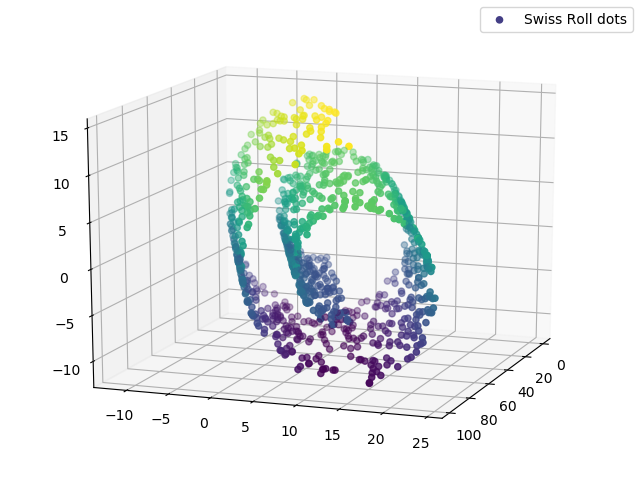
\includegraphics[width=.5\textwidth]{SwissRoll1.png}}\hfill
	\subfloat[Swiss Roll数据降维结果]{%
		\label{fig:PCA1}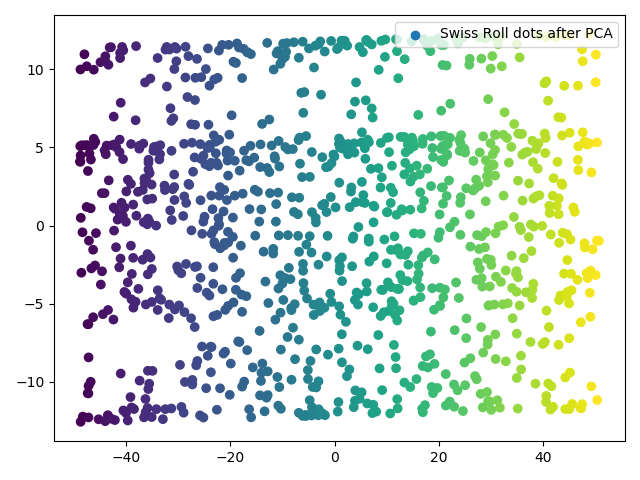
\includegraphics[width=.5\textwidth]{PCA1.png}}
	\caption{$number=1000, noise=0, height=100$生成的Swiss Roll数据并降维结果}\label{fig:Swiss1}
\end{figure}

当$number=2000, noise=0, height=10$时,生成的数据图像如图(\ref{fig:SwissRoll2})所示,降维的结果如图(\ref{fig:PCA2})所示。

\begin{figure}[h]
	\centering
	\subfloat[Swiss Roll数据]{%
		\label{fig:SwissRoll2}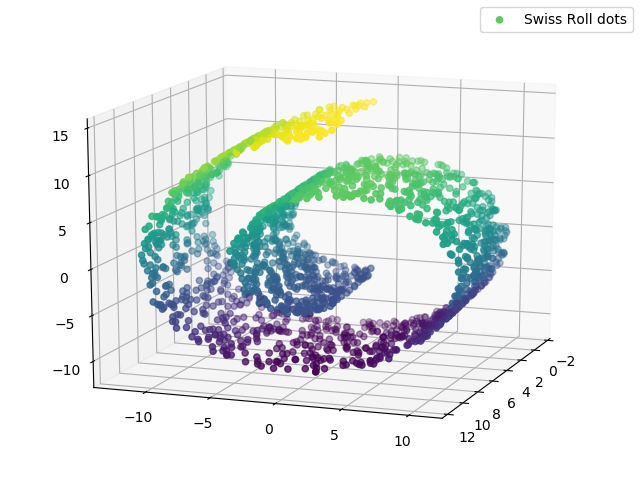
\includegraphics[width=.5\textwidth]{SwissRoll2.png}}\hfill
	\subfloat[Swiss Roll数据降维结果]{%
		\label{fig:PCA2}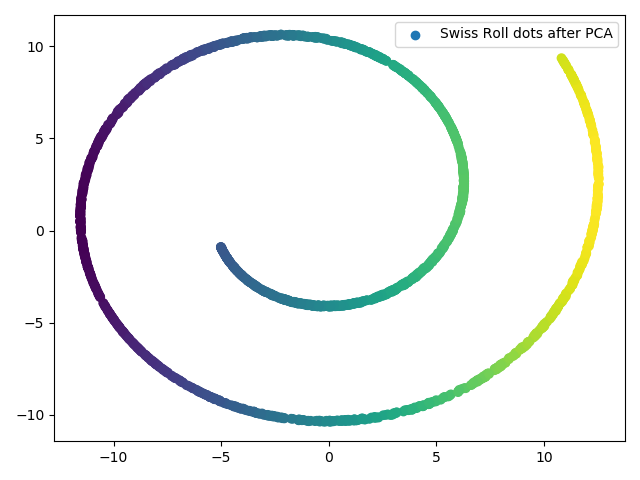
\includegraphics[width=.5\textwidth]{PCA2.png}}
	\caption{$number=2000, noise=0, height=10$生成的Swiss Roll数据并降维结果}\label{fig:Swiss2}
\end{figure}


当$number=2000, noise=1, height=10$时,生成的数据图像如图(\ref{fig:SwissRoll3})所示,降维的结果如图(\ref{fig:PCA3})所示。


\begin{figure}[h]
	\centering
	\subfloat[Swiss Roll数据]{%
		\label{fig:SwissRoll3}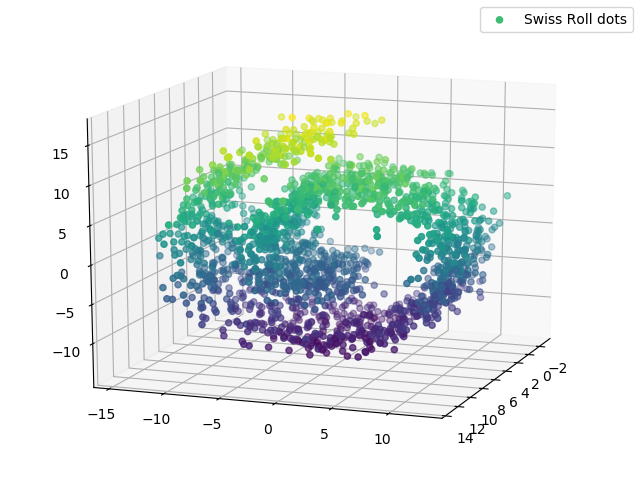
\includegraphics[width=.5\textwidth]{SwissRoll3.png}}\hfill
	\subfloat[Swiss Roll数据降维结果]{%
		\label{fig:PCA3}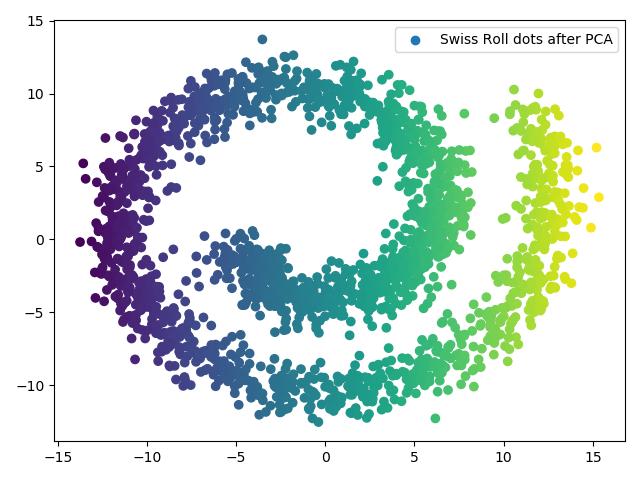
\includegraphics[width=.5\textwidth]{PCA3.png}}
	\caption{$number=2000, noise=1, height=10$生成的Swiss Roll数据并降维结果}\label{fig:Swiss3}
\end{figure}


\subsection{生成数据结果分析}

从上面三次实验可以看出,不同的height对于Swiss Roll数据主成分提取的影响不同。当height=10较小时,Swiss Roll数据的结果较“薄”,涡旋状的正投影方差较大,所以结果为涡旋状的正投影,如图(\ref{fig:PCA2})所示;当height=100较大时,Swiss Roll数据的结果较“厚”,矩形的侧投影方差较大,所以结果为矩形的侧投影,如图(\ref{fig:PCA1})所示。

当height=10时,对所有的数据点加上了noise=1的噪声,尽管正投影面变得不再光滑,但是可以看出依然是旋涡状,如图(\ref{fig:PCA3})所示。

\subsection{对人脸数据的降维}

人脸压缩数据来自数据集WIDER FACE人脸检测基准数据集,从中选择了特征较明显的9张图片,原图如图(\ref{fig:face1})所示,原图片的像素是255*255,为了加快计算速度,使用opencv自带的函数,对图片进行大小重构,为50*50,再进行降维操作,之后分别计算不同维度降维的信噪比。

对图片进行降维,降维后维度为8,图片结果如图(\ref{fig:face8}),计算信噪比如图(\ref{fig:loss8})所示。

\begin{figure}[htb]
	\centering
	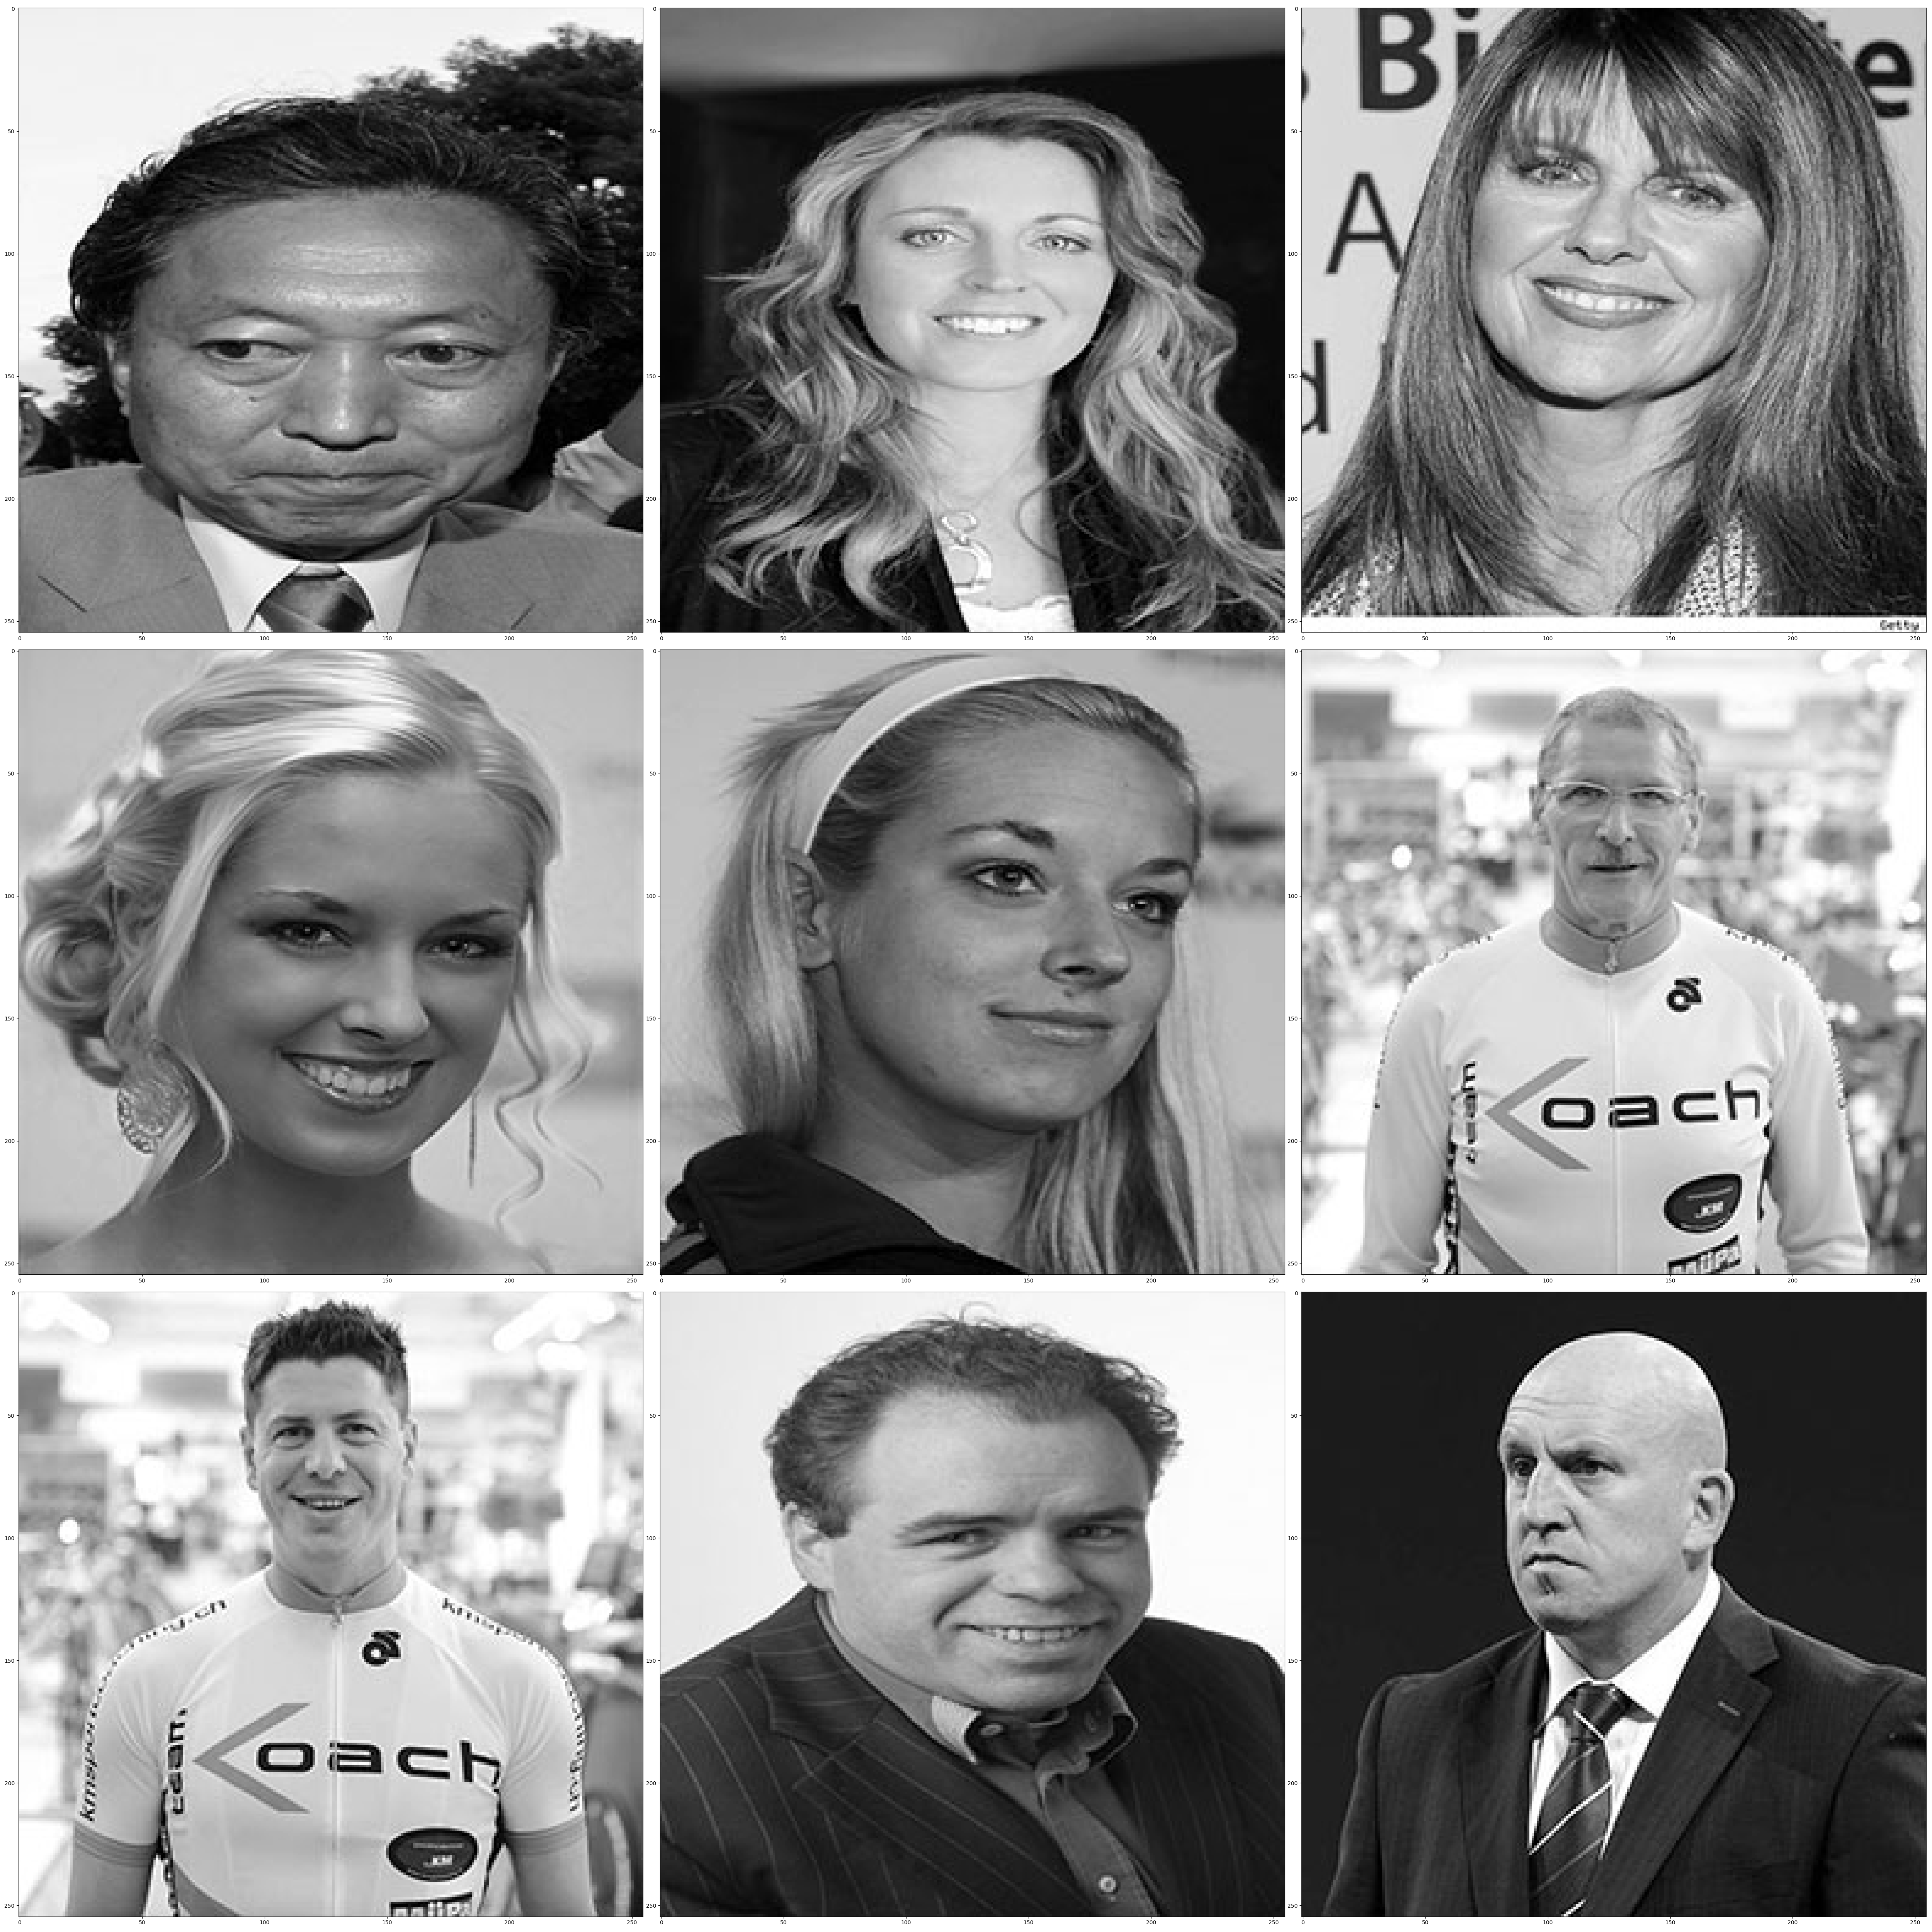
\includegraphics[width=.6\textwidth]{face1.png}
	\caption{人脸数据原图}
	\label{fig:face1}
\end{figure}

\begin{figure}[htb]
	\centering
	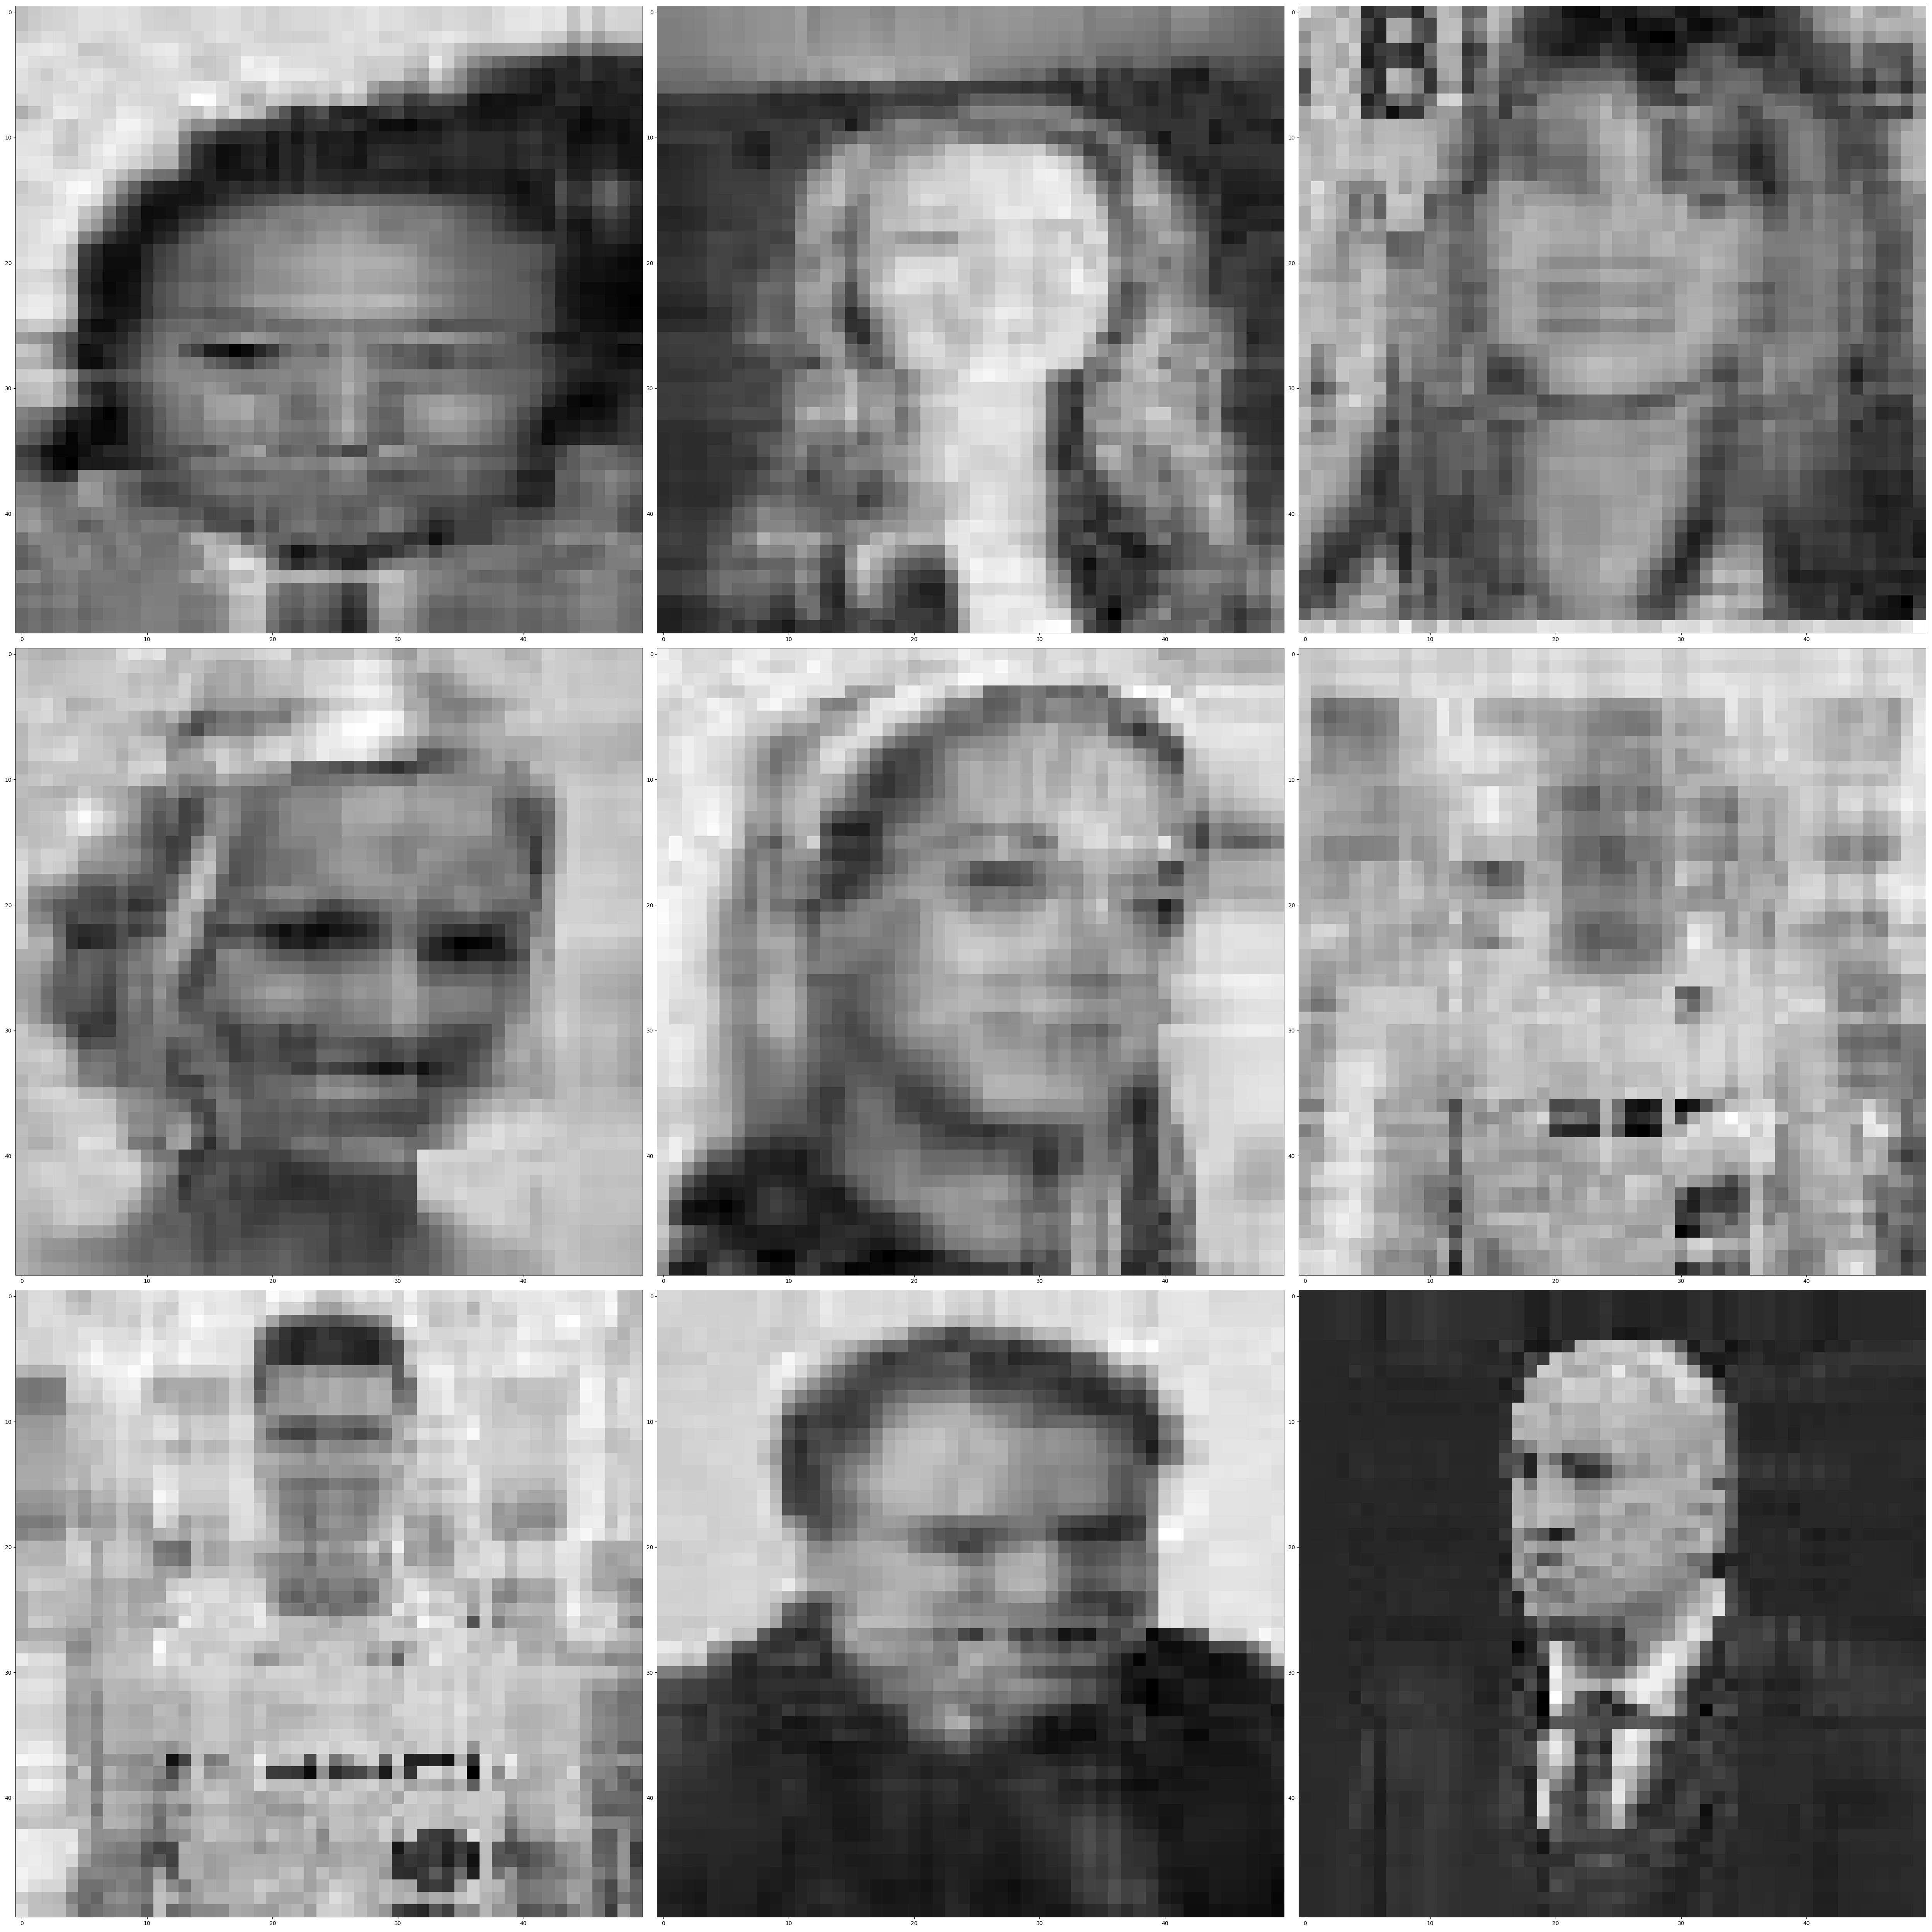
\includegraphics[width=.6\textwidth]{face8.png}
	\caption{人脸数据降维维度为8的结果}
	\label{fig:face8}
\end{figure}

\begin{figure}[htb]
	\centering
	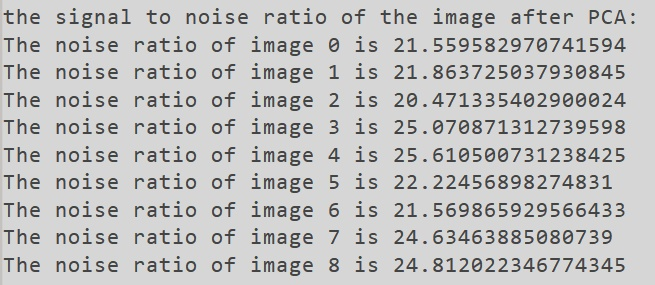
\includegraphics[width=.6\textwidth]{loss8.jpeg}
	\caption{人脸数据降维维度为8的信噪比结果}
	\label{fig:loss8}
\end{figure}

对图片进行降维,降维后维度为5,图片结果如图(\ref{fig:face5}),计算信噪比如图(\ref{fig:loss5})所示。

\begin{figure}[htb]
	\centering
	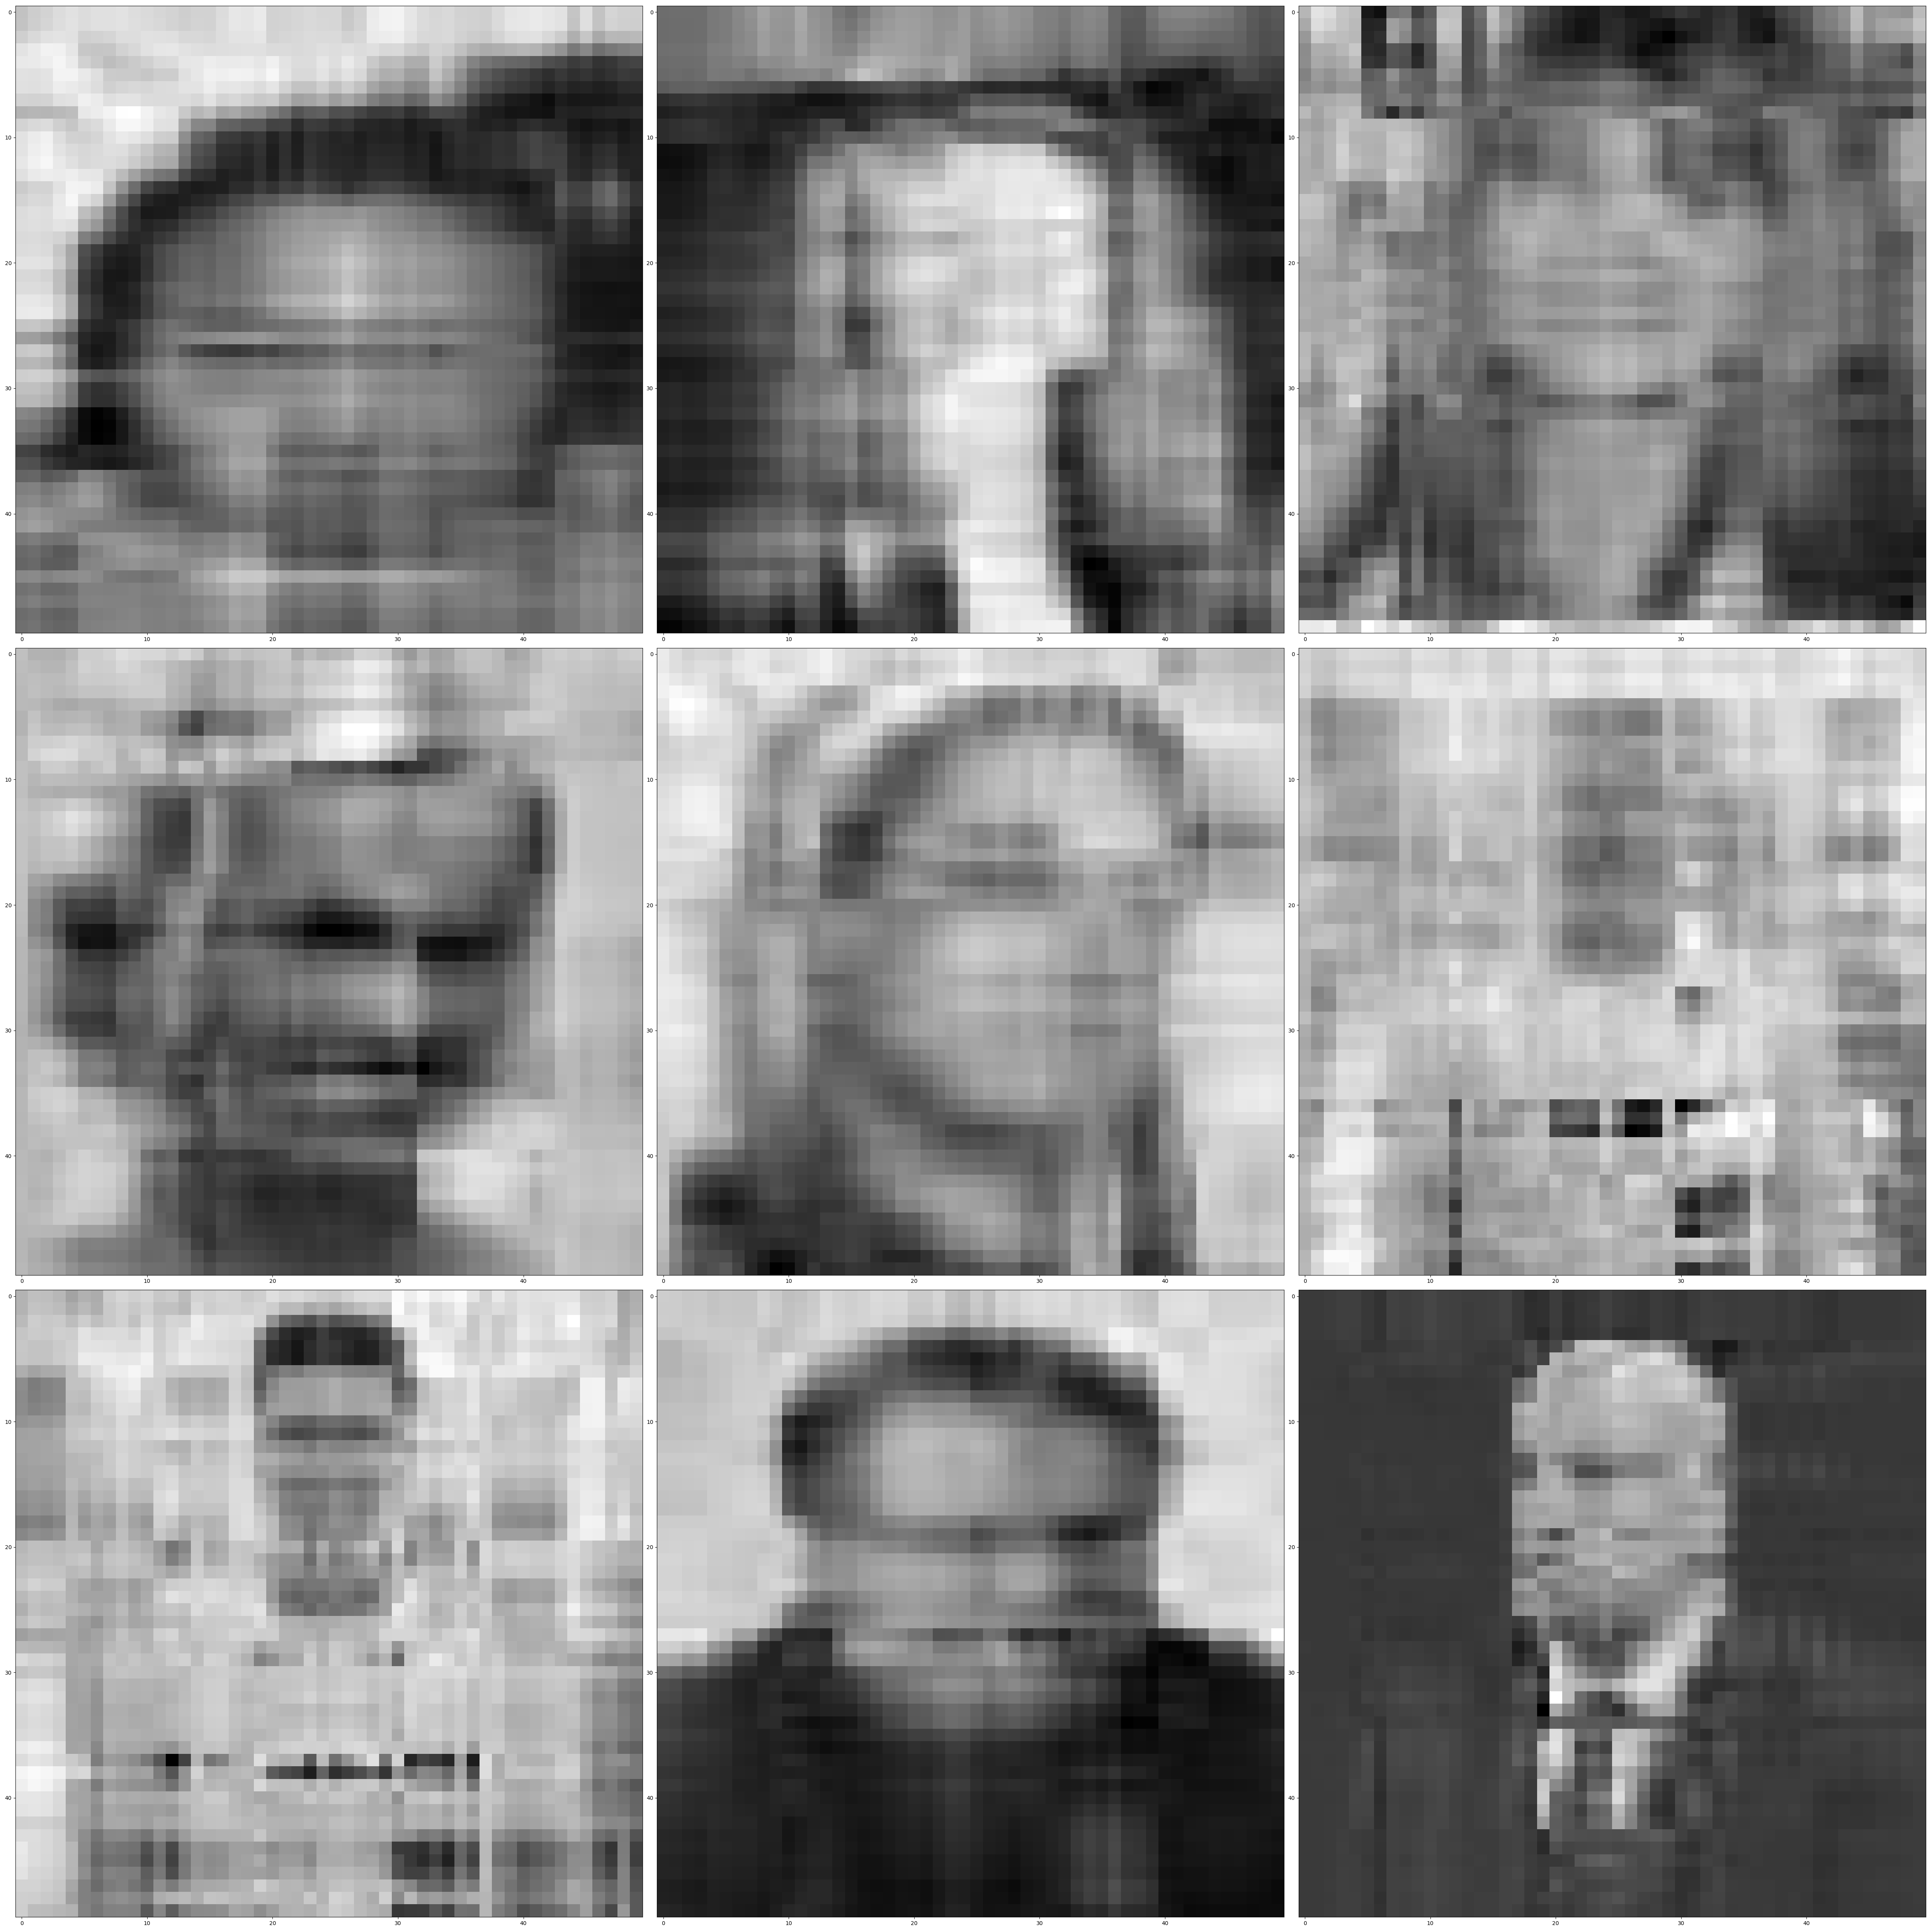
\includegraphics[width=.6\textwidth]{face5.png}
	\caption{人脸数据降维维度为5的结果}
	\label{fig:face5}
\end{figure}

\begin{figure}[htb]
	\centering
	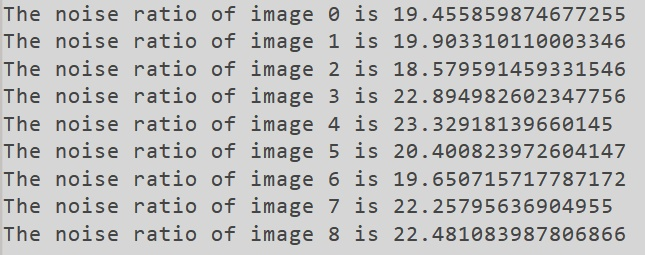
\includegraphics[width=.6\textwidth]{loss5.jpeg}
	\caption{人脸数据降维维度为5的信噪比结果}
	\label{fig:loss5}
\end{figure}


对图片进行降维,降维后维度为3,图片结果如图(\ref{fig:face3}),计算信噪比如图(\ref{fig:loss3})所示。

\begin{figure}[htb]
	\centering
	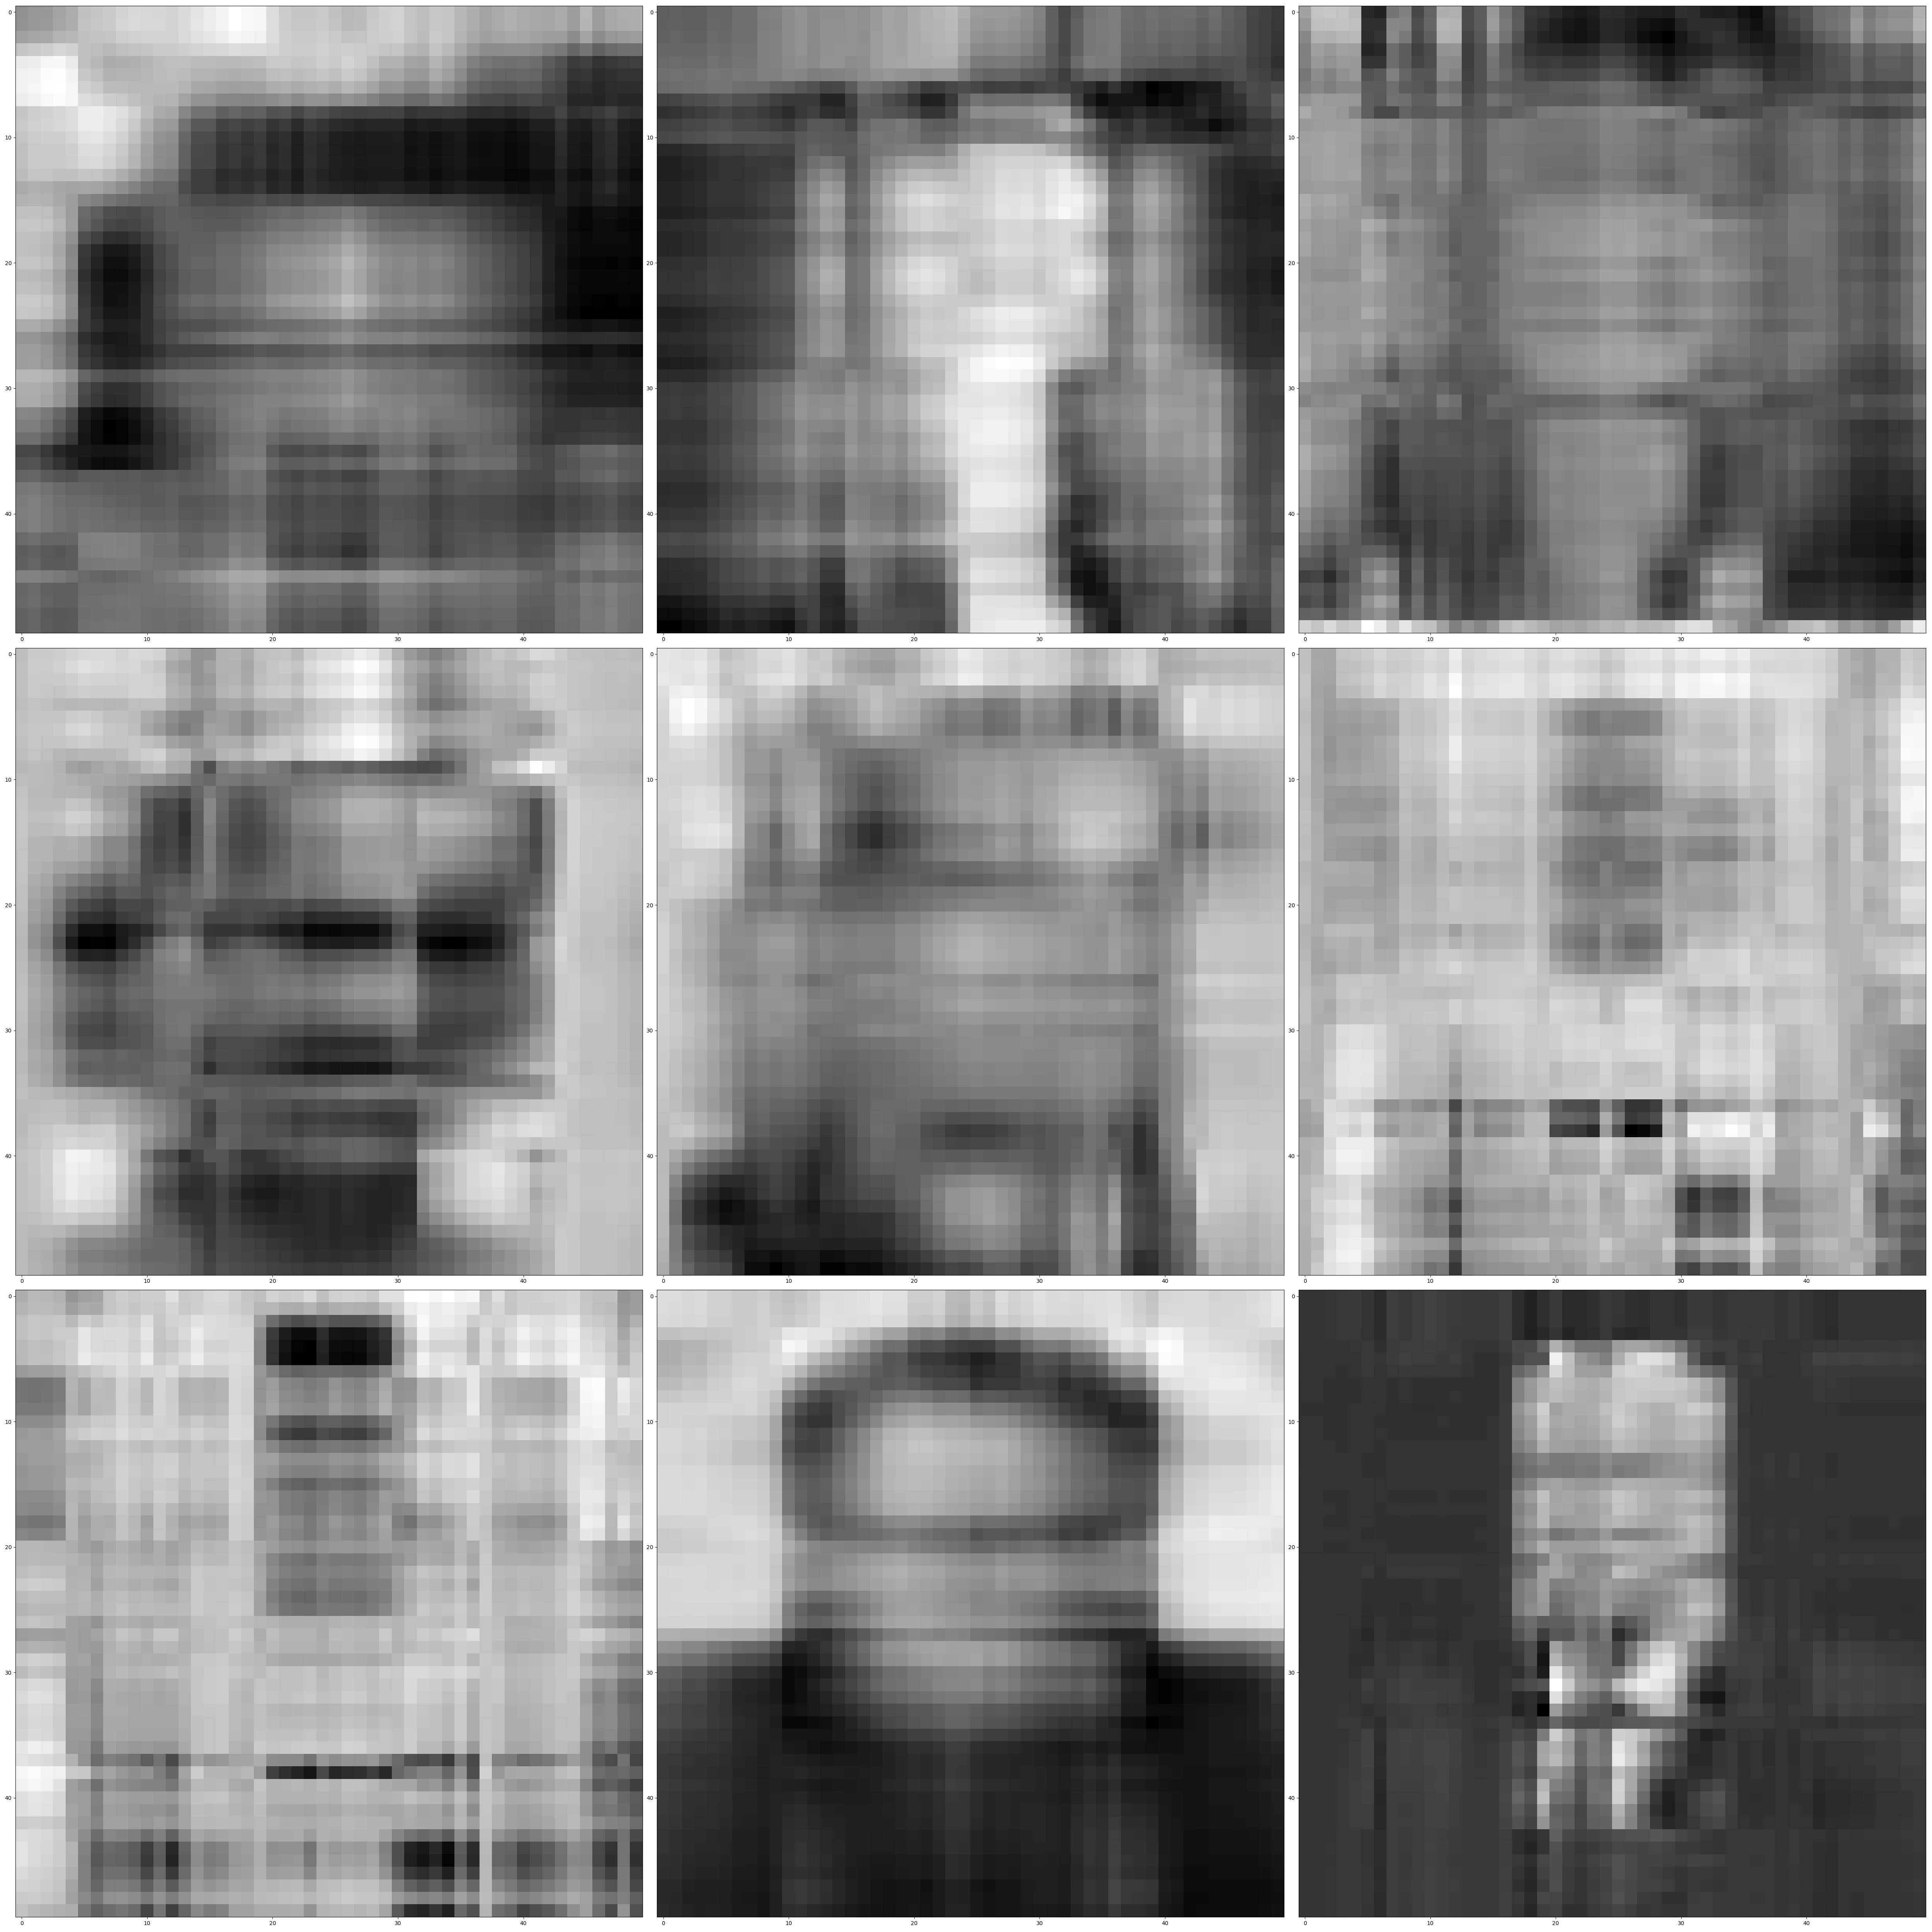
\includegraphics[width=.6\textwidth]{face3.png}
	\caption{人脸数据降维维度为3的结果}
	\label{fig:face3}
\end{figure}

\begin{figure}[htb]
	\centering
	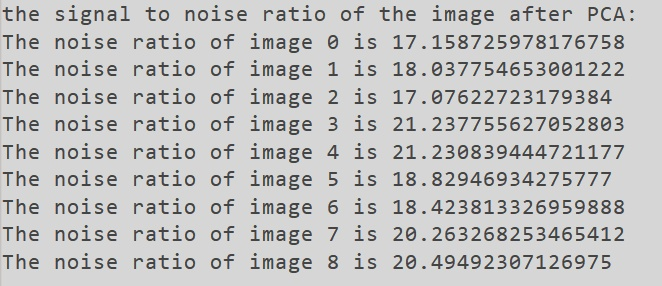
\includegraphics[width=.6\textwidth]{loss3.jpeg}
	\caption{人脸数据降维维度为3的信噪比结果}
	\label{fig:loss3}
\end{figure}

\subsection{对人脸数据降维分析}

可以看出,随着降维维度的降低,人脸数据逐渐变得模糊,信噪比也越来越低,可以看到,随着降维空间的维数提高,对于源数据的信息保留的更加全面。

\section{实验结论}

\begin{enumerate}
\item PCA算法中舍弃了$n-d$个最小的特征值对应的特征向量,一定会导致低维空间与高维空间不同,但是通过这种方式提取出了数据的主成分,对数据做了一定程度的压缩,压缩比例随降维维数的降低而提高;
\item PCA不仅将数据压缩到低维,并且将降维之后的各维特征相互独立;
\item 通过对各维度向量计算向量均值,通过向量减法将新样本进行中心化来减小向量在不同维度上分布不均匀对降维想过的影响.
\end{enumerate}

\renewcommand\refname{参考文献}
 
\begin{thebibliography}{2}
\bibitem{book:li}
李航, 统计学习方法(2019.3).

\bibitem{book:zhou}
周志华, 机器学习(2016.1).

\bibitem{url:bank}
\href{http://shuoyang1213.me/WIDERFACE}{WIDER FACE: A Face Detection Benchmark. (2017.3) [Data set]}.
\end{thebibliography}

\newpage
\begin{appendices}

\section{生成Swiss Roll数据--generate\_data.py}\label{app:Swiss Roll}
\begin{lstlisting}[language=python]
import numpy as np


def rotation_transformation(data, theta=0, axis='x'):
    if axis == 'x':
        rotation_matrix = [[1, 0, 0], [0, np.cos(theta), -np.sin(theta)], [0, np.sin(theta), np.cos(theta)]]
    elif axis == 'y':
        rotation_matrix = [[np.cos(theta), 0, np.sin(theta)], [0, 1, 0], [-np.sin(theta), 0, np.cos(theta)]]
    elif axis == 'z':
        rotation_matrix = [[np.cos(theta), -np.sin(theta), 0], [np.sin(theta), np.cos(theta), 0], [0, 0, 1]]
    else:
        print("wrong input")
        return data
    return np.dot(rotation_matrix, data)


def generate_data(number, noise, height):
    tt1 = (3 * np.pi / 2) * (1 + 2 * np.random.rand(1, number))
    x = tt1 * np.cos(tt1)
    y = height * np.random.rand(1, number)
    z = tt1 * np.sin(tt1)
    X = np.concatenate((x, y, z))
    X += noise * np.random.randn(3, number)
    X = rotation_transformation(X, 30, 'z')
    return X.T

\end{lstlisting}

\section{PCA主成分分析法算法--PCA.py}\label{app:gmm}
\begin{lstlisting}[language=python]
import numpy as np


class PCA(object):

    def __init__(self, data, k):
        self.data = data
        self.k = k
        self.rows, self.columns = self.data.shape

    def pca(self):
        data_mean = np.sum(self.data, axis=0) / self.rows
        central_data = self.data - data_mean
        cov_matrix = central_data.T.dot(central_data)
        eigen_values, eigen_vector = np.linalg.eig(cov_matrix)
        eigen_value_sort = np.argsort(eigen_values)
        eigen_result = eigen_vector[:, eigen_value_sort[:-(self.k + 1):-1]]
        return central_data, eigen_result, data_mean

\end{lstlisting}

\section{主程序--lab4\_main.py}\label{app:data}
\begin{lstlisting}[language=python]
from src.PCA import *
from src.generate_data import *
from src.generate_picture import *
from src.dimensionality_reduction_image import *


def test_pca(data):
    generate_3_dimension_picture(data)
    central_data, eig_vector, data_mean = PCA(data, 2).pca()
    pca_data = np.dot(central_data, eig_vector)
    generate_2_dimension_picture(pca_data)


def test_image_data_set():
    data = read_image_data()
    image_number, image_feature = data[0].shape
    print(data.shape)
    central_data = []
    eig_vector = []
    data_mean = []
    pca_data = []
    rebuild_data = []
    for i in range(len(data)):
        central_data_i, eig_vector_i, data_mean_i = PCA(data[i], 8).pca()
        central_data.append(central_data_i)
        eig_vector.append(eig_vector_i)
        data_mean.append(data_mean_i)
        print(eig_vector[i])
        eig_vector_i = np.real(eig_vector_i)
        pca_data.append(np.dot(central_data_i, eig_vector_i))
        # print(pca_data)
        rebuild_data.append(np.dot(pca_data[i], eig_vector[i].T) + data_mean[i])
    plt.figure(figsize=(50, 50))
    for i in range(len(data)):
        plt.subplot(3, 3, i + 1)
        plt.imshow(rebuild_data[i], cmap=plt.cm.gray)
    plt.show()

    print("the signal to noise ratio of the image after PCA:")
    for i in range(len(data)):
        ratio = calculate_noise_ratio(data[i], rebuild_data[i])
        print('The noise ratio of image ' + str(i) + ' is ' + str(ratio))


def test_single_picture():
    data = read_image_data()
    image_number, image_feature = data.shape
    print(data.shape)
    central_data, eig_vector, data_mean = PCA(data, 20).pca()
    print(eig_vector)
    eig_vector = np.real(eig_vector)
    pca_data = np.dot(central_data, eig_vector)
    rebuild_data = np.dot(pca_data, eig_vector.T) + data_mean
    plt.figure(figsize=(50, 50))
    plt.imshow(rebuild_data)
    plt.show()


def main():
    data_1 = generate_data(1000, 0, 100)
    # print(np.shape(data_1))
    data_2 = generate_data(2000, 0, 10)
    data_3 = generate_data(2000, 1, 10)

    test_pca(data_1)
    test_pca(data_2)
    test_pca(data_3)

    test_image_data_set()


if __name__ == '__main__':
    main()


\end{lstlisting}

\section{对图片降维并计算信噪比--dimensionality\_reduction\_image.py}\label{app:main}
\begin{lstlisting}[language=python]
import matplotlib.pyplot as plt
import numpy as np
import cv2 as cv
import os


def read_image_data():
    file_dir_path = '../data/'
    file_list = os.listdir(file_dir_path)
    image_data = []
    plt.figure(figsize=(50, 50))
    i = 1
    for file in file_list:
        file_path = os.path.join(file_dir_path, file)
        print("open figure " + file_path)
        plt.subplot(3, 3, i)
        with open(file_path) as f:
            img = cv.imread(file_path, cv.IMREAD_GRAYSCALE)
            print(img.shape)
            img = cv.resize(img, (50, 50), interpolation=cv.INTER_NEAREST)
            print(img.shape)
            # cv.imshow("sdg", img)
            # cv.waitKey(0)
            # cv.destroyAllWindows()
            # height, width = img.shape
            # img_temp = img.reshape(height * width)
            # data.append(img_temp)
            data = np.asarray(img)
            image_data.append(data)
            plt.imshow(img, cmap=plt.cm.gray)
            # cv.imshow("sg", img)
            # cv.waitKey(0)
            # cv.destroyAllWindows()
        i += 1
    plt.show()
    return np.asarray(image_data)


def calculate_noise_ratio(img_1, img_2):
    noise = np.mean(np.square(img_1 / 255. - img_2 / 255.))
    if noise < 1e-10:
        return 100
    return 20 * np.log10(1 / np.sqrt(noise))


\end{lstlisting}


\end{appendices}

\end{document}
